\section{Can you remember a time that you were upset as a child?}
I remember several times that I was upset as a child.
An early one was waking up during the night and bumping my head.
I bumped my head because I found myself under the bed.
So why was I there? I don't know perhaps I had a nightmare or bad dream.
So I crawled out from under the bed and climbed back in beside my sister.
\begin{figure}
\centering
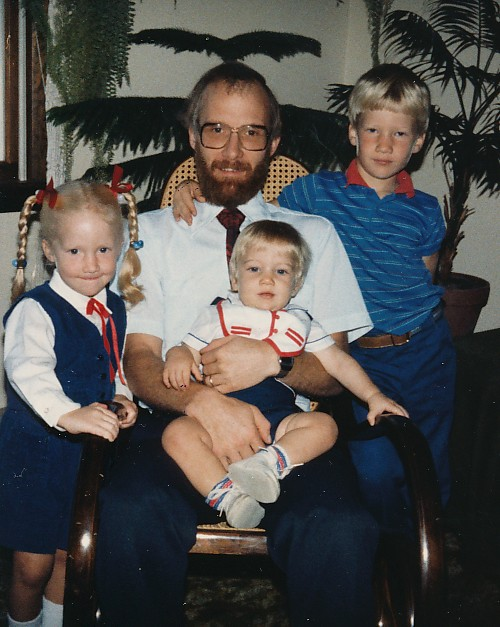
\includegraphics[width=0.75\textwidth]{childhood/3.jpg}
\caption{
Three sisters at Aunties house
}
\end{figure}

Another time was finding my little brother holding a paring knife.
When I thought I would take it from him the knife cut the tip of my left pointer finger.
The cut called for a trip to a doctor and three stitches to hold it together.
The wound healed fine and left me with a scar.
\begin{figure}
\centering
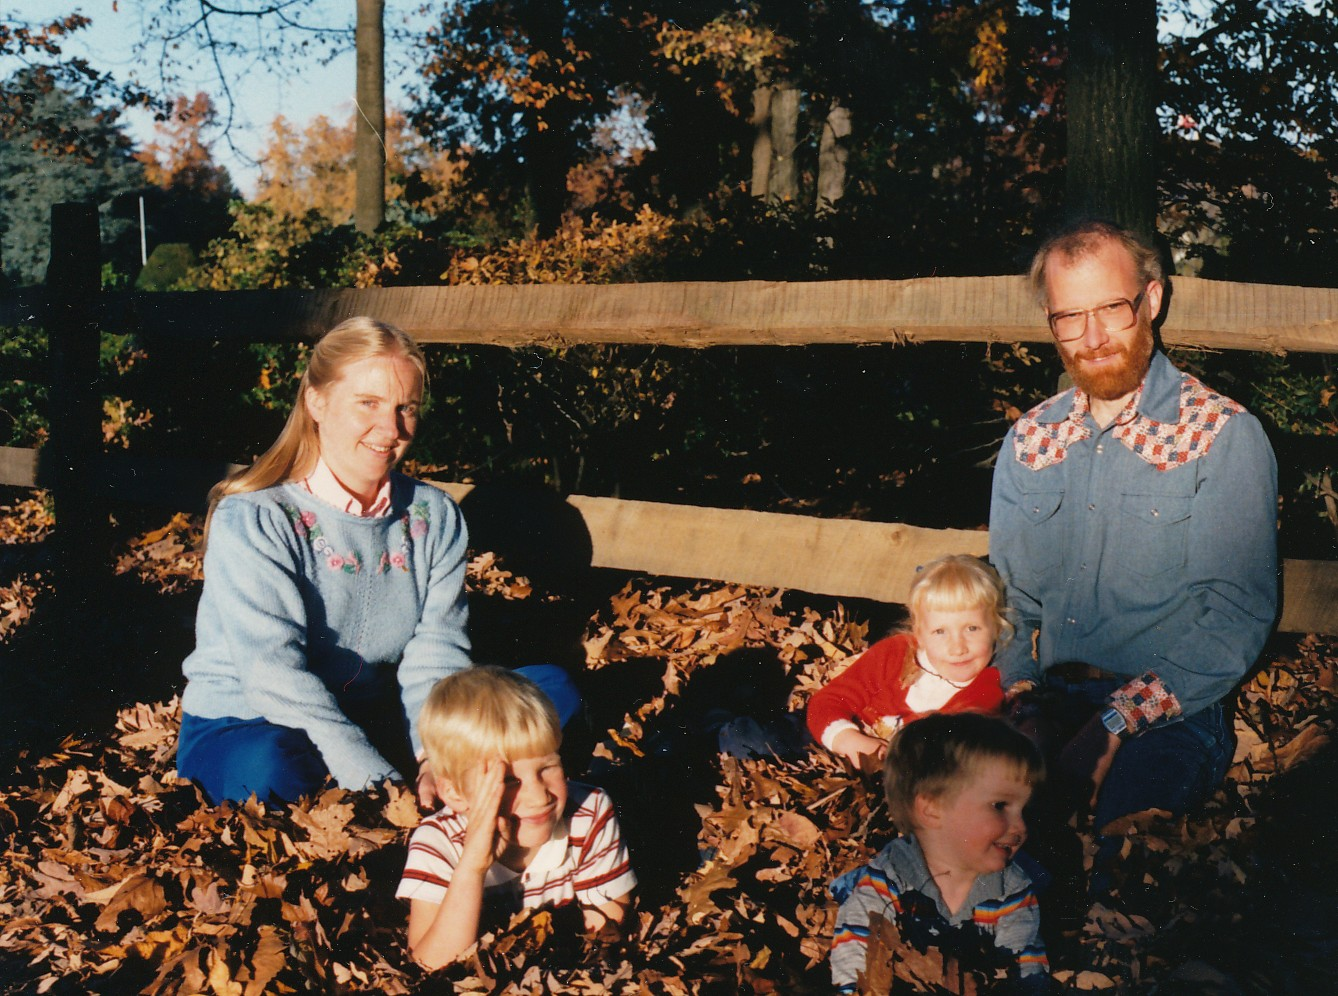
\includegraphics[width=0.75\textwidth]{childhood/4.jpg}
\caption{
Lois and Mary with a kitten and dog, Nicky
}
\end{figure}

Another kind of memory came to me from my elementary school years.
This involved an older brother.
He operated the milking machines and Mary and I were to prep the cows and carry the buckets full of milk to the milk house.
Mary most often washed the cows udders and I helped by putting a strap over the cow's back.
The milking machine was hooked on the strap.
In between these jobs we would play outside the barn.
If we were slow in getting back inside and getting the jobs done he would occasionally hit us with the rubber hose of the milking machine.
He most often hit our legs.
I did not like him for doing this to us.
